
\documentclass{article} % For LaTeX2e
\usepackage{iclr2020_conference,times}

% Optional math commands from https://github.com/goodfeli/dlbook_notation.
%%%%% NEW MATH DEFINITIONS %%%%%

\usepackage{amsmath,amsfonts,bm}

% Mark sections of captions for referring to divisions of figures
\newcommand{\figleft}{{\em (Left)}}
\newcommand{\figcenter}{{\em (Center)}}
\newcommand{\figright}{{\em (Right)}}
\newcommand{\figtop}{{\em (Top)}}
\newcommand{\figbottom}{{\em (Bottom)}}
\newcommand{\captiona}{{\em (a)}}
\newcommand{\captionb}{{\em (b)}}
\newcommand{\captionc}{{\em (c)}}
\newcommand{\captiond}{{\em (d)}}

% Highlight a newly defined term
\newcommand{\newterm}[1]{{\bf #1}}


% Figure reference, lower-case.
\def\figref#1{figure~\ref{#1}}
% Figure reference, capital. For start of sentence
\def\Figref#1{Figure~\ref{#1}}
\def\twofigref#1#2{figures \ref{#1} and \ref{#2}}
\def\quadfigref#1#2#3#4{figures \ref{#1}, \ref{#2}, \ref{#3} and \ref{#4}}
% Section reference, lower-case.
\def\secref#1{section~\ref{#1}}
% Section reference, capital.
\def\Secref#1{Section~\ref{#1}}
% Reference to two sections.
\def\twosecrefs#1#2{sections \ref{#1} and \ref{#2}}
% Reference to three sections.
\def\secrefs#1#2#3{sections \ref{#1}, \ref{#2} and \ref{#3}}
% Reference to an equation, lower-case.
\def\eqref#1{equation~\ref{#1}}
% Reference to an equation, upper case
\def\Eqref#1{Equation~\ref{#1}}
% A raw reference to an equation---avoid using if possible
\def\plaineqref#1{\ref{#1}}
% Reference to a chapter, lower-case.
\def\chapref#1{chapter~\ref{#1}}
% Reference to an equation, upper case.
\def\Chapref#1{Chapter~\ref{#1}}
% Reference to a range of chapters
\def\rangechapref#1#2{chapters\ref{#1}--\ref{#2}}
% Reference to an algorithm, lower-case.
\def\algref#1{algorithm~\ref{#1}}
% Reference to an algorithm, upper case.
\def\Algref#1{Algorithm~\ref{#1}}
\def\twoalgref#1#2{algorithms \ref{#1} and \ref{#2}}
\def\Twoalgref#1#2{Algorithms \ref{#1} and \ref{#2}}
% Reference to a part, lower case
\def\partref#1{part~\ref{#1}}
% Reference to a part, upper case
\def\Partref#1{Part~\ref{#1}}
\def\twopartref#1#2{parts \ref{#1} and \ref{#2}}

\def\ceil#1{\lceil #1 \rceil}
\def\floor#1{\lfloor #1 \rfloor}
\def\1{\bm{1}}
\newcommand{\train}{\mathcal{D}}
\newcommand{\valid}{\mathcal{D_{\mathrm{valid}}}}
\newcommand{\test}{\mathcal{D_{\mathrm{test}}}}

\def\eps{{\epsilon}}


% Random variables
\def\reta{{\textnormal{$\eta$}}}
\def\ra{{\textnormal{a}}}
\def\rb{{\textnormal{b}}}
\def\rc{{\textnormal{c}}}
\def\rd{{\textnormal{d}}}
\def\re{{\textnormal{e}}}
\def\rf{{\textnormal{f}}}
\def\rg{{\textnormal{g}}}
\def\rh{{\textnormal{h}}}
\def\ri{{\textnormal{i}}}
\def\rj{{\textnormal{j}}}
\def\rk{{\textnormal{k}}}
\def\rl{{\textnormal{l}}}
% rm is already a command, just don't name any random variables m
\def\rn{{\textnormal{n}}}
\def\ro{{\textnormal{o}}}
\def\rp{{\textnormal{p}}}
\def\rq{{\textnormal{q}}}
\def\rr{{\textnormal{r}}}
\def\rs{{\textnormal{s}}}
\def\rt{{\textnormal{t}}}
\def\ru{{\textnormal{u}}}
\def\rv{{\textnormal{v}}}
\def\rw{{\textnormal{w}}}
\def\rx{{\textnormal{x}}}
\def\ry{{\textnormal{y}}}
\def\rz{{\textnormal{z}}}

% Random vectors
\def\rvepsilon{{\mathbf{\epsilon}}}
\def\rvtheta{{\mathbf{\theta}}}
\def\rva{{\mathbf{a}}}
\def\rvb{{\mathbf{b}}}
\def\rvc{{\mathbf{c}}}
\def\rvd{{\mathbf{d}}}
\def\rve{{\mathbf{e}}}
\def\rvf{{\mathbf{f}}}
\def\rvg{{\mathbf{g}}}
\def\rvh{{\mathbf{h}}}
\def\rvu{{\mathbf{i}}}
\def\rvj{{\mathbf{j}}}
\def\rvk{{\mathbf{k}}}
\def\rvl{{\mathbf{l}}}
\def\rvm{{\mathbf{m}}}
\def\rvn{{\mathbf{n}}}
\def\rvo{{\mathbf{o}}}
\def\rvp{{\mathbf{p}}}
\def\rvq{{\mathbf{q}}}
\def\rvr{{\mathbf{r}}}
\def\rvs{{\mathbf{s}}}
\def\rvt{{\mathbf{t}}}
\def\rvu{{\mathbf{u}}}
\def\rvv{{\mathbf{v}}}
\def\rvw{{\mathbf{w}}}
\def\rvx{{\mathbf{x}}}
\def\rvy{{\mathbf{y}}}
\def\rvz{{\mathbf{z}}}

% Elements of random vectors
\def\erva{{\textnormal{a}}}
\def\ervb{{\textnormal{b}}}
\def\ervc{{\textnormal{c}}}
\def\ervd{{\textnormal{d}}}
\def\erve{{\textnormal{e}}}
\def\ervf{{\textnormal{f}}}
\def\ervg{{\textnormal{g}}}
\def\ervh{{\textnormal{h}}}
\def\ervi{{\textnormal{i}}}
\def\ervj{{\textnormal{j}}}
\def\ervk{{\textnormal{k}}}
\def\ervl{{\textnormal{l}}}
\def\ervm{{\textnormal{m}}}
\def\ervn{{\textnormal{n}}}
\def\ervo{{\textnormal{o}}}
\def\ervp{{\textnormal{p}}}
\def\ervq{{\textnormal{q}}}
\def\ervr{{\textnormal{r}}}
\def\ervs{{\textnormal{s}}}
\def\ervt{{\textnormal{t}}}
\def\ervu{{\textnormal{u}}}
\def\ervv{{\textnormal{v}}}
\def\ervw{{\textnormal{w}}}
\def\ervx{{\textnormal{x}}}
\def\ervy{{\textnormal{y}}}
\def\ervz{{\textnormal{z}}}

% Random matrices
\def\rmA{{\mathbf{A}}}
\def\rmB{{\mathbf{B}}}
\def\rmC{{\mathbf{C}}}
\def\rmD{{\mathbf{D}}}
\def\rmE{{\mathbf{E}}}
\def\rmF{{\mathbf{F}}}
\def\rmG{{\mathbf{G}}}
\def\rmH{{\mathbf{H}}}
\def\rmI{{\mathbf{I}}}
\def\rmJ{{\mathbf{J}}}
\def\rmK{{\mathbf{K}}}
\def\rmL{{\mathbf{L}}}
\def\rmM{{\mathbf{M}}}
\def\rmN{{\mathbf{N}}}
\def\rmO{{\mathbf{O}}}
\def\rmP{{\mathbf{P}}}
\def\rmQ{{\mathbf{Q}}}
\def\rmR{{\mathbf{R}}}
\def\rmS{{\mathbf{S}}}
\def\rmT{{\mathbf{T}}}
\def\rmU{{\mathbf{U}}}
\def\rmV{{\mathbf{V}}}
\def\rmW{{\mathbf{W}}}
\def\rmX{{\mathbf{X}}}
\def\rmY{{\mathbf{Y}}}
\def\rmZ{{\mathbf{Z}}}

% Elements of random matrices
\def\ermA{{\textnormal{A}}}
\def\ermB{{\textnormal{B}}}
\def\ermC{{\textnormal{C}}}
\def\ermD{{\textnormal{D}}}
\def\ermE{{\textnormal{E}}}
\def\ermF{{\textnormal{F}}}
\def\ermG{{\textnormal{G}}}
\def\ermH{{\textnormal{H}}}
\def\ermI{{\textnormal{I}}}
\def\ermJ{{\textnormal{J}}}
\def\ermK{{\textnormal{K}}}
\def\ermL{{\textnormal{L}}}
\def\ermM{{\textnormal{M}}}
\def\ermN{{\textnormal{N}}}
\def\ermO{{\textnormal{O}}}
\def\ermP{{\textnormal{P}}}
\def\ermQ{{\textnormal{Q}}}
\def\ermR{{\textnormal{R}}}
\def\ermS{{\textnormal{S}}}
\def\ermT{{\textnormal{T}}}
\def\ermU{{\textnormal{U}}}
\def\ermV{{\textnormal{V}}}
\def\ermW{{\textnormal{W}}}
\def\ermX{{\textnormal{X}}}
\def\ermY{{\textnormal{Y}}}
\def\ermZ{{\textnormal{Z}}}

% Vectors
\def\vzero{{\bm{0}}}
\def\vone{{\bm{1}}}
\def\vmu{{\bm{\mu}}}
\def\vtheta{{\bm{\theta}}}
\def\va{{\bm{a}}}
\def\vb{{\bm{b}}}
\def\vc{{\bm{c}}}
\def\vd{{\bm{d}}}
\def\ve{{\bm{e}}}
\def\vf{{\bm{f}}}
\def\vg{{\bm{g}}}
\def\vh{{\bm{h}}}
\def\vi{{\bm{i}}}
\def\vj{{\bm{j}}}
\def\vk{{\bm{k}}}
\def\vl{{\bm{l}}}
\def\vm{{\bm{m}}}
\def\vn{{\bm{n}}}
\def\vo{{\bm{o}}}
\def\vp{{\bm{p}}}
\def\vq{{\bm{q}}}
\def\vr{{\bm{r}}}
\def\vs{{\bm{s}}}
\def\vt{{\bm{t}}}
\def\vu{{\bm{u}}}
\def\vv{{\bm{v}}}
\def\vw{{\bm{w}}}
\def\vx{{\bm{x}}}
\def\vy{{\bm{y}}}
\def\vz{{\bm{z}}}

% Elements of vectors
\def\evalpha{{\alpha}}
\def\evbeta{{\beta}}
\def\evepsilon{{\epsilon}}
\def\evlambda{{\lambda}}
\def\evomega{{\omega}}
\def\evmu{{\mu}}
\def\evpsi{{\psi}}
\def\evsigma{{\sigma}}
\def\evtheta{{\theta}}
\def\eva{{a}}
\def\evb{{b}}
\def\evc{{c}}
\def\evd{{d}}
\def\eve{{e}}
\def\evf{{f}}
\def\evg{{g}}
\def\evh{{h}}
\def\evi{{i}}
\def\evj{{j}}
\def\evk{{k}}
\def\evl{{l}}
\def\evm{{m}}
\def\evn{{n}}
\def\evo{{o}}
\def\evp{{p}}
\def\evq{{q}}
\def\evr{{r}}
\def\evs{{s}}
\def\evt{{t}}
\def\evu{{u}}
\def\evv{{v}}
\def\evw{{w}}
\def\evx{{x}}
\def\evy{{y}}
\def\evz{{z}}

% Matrix
\def\mA{{\bm{A}}}
\def\mB{{\bm{B}}}
\def\mC{{\bm{C}}}
\def\mD{{\bm{D}}}
\def\mE{{\bm{E}}}
\def\mF{{\bm{F}}}
\def\mG{{\bm{G}}}
\def\mH{{\bm{H}}}
\def\mI{{\bm{I}}}
\def\mJ{{\bm{J}}}
\def\mK{{\bm{K}}}
\def\mL{{\bm{L}}}
\def\mM{{\bm{M}}}
\def\mN{{\bm{N}}}
\def\mO{{\bm{O}}}
\def\mP{{\bm{P}}}
\def\mQ{{\bm{Q}}}
\def\mR{{\bm{R}}}
\def\mS{{\bm{S}}}
\def\mT{{\bm{T}}}
\def\mU{{\bm{U}}}
\def\mV{{\bm{V}}}
\def\mW{{\bm{W}}}
\def\mX{{\bm{X}}}
\def\mY{{\bm{Y}}}
\def\mZ{{\bm{Z}}}
\def\mBeta{{\bm{\beta}}}
\def\mPhi{{\bm{\Phi}}}
\def\mLambda{{\bm{\Lambda}}}
\def\mSigma{{\bm{\Sigma}}}

% Tensor
\DeclareMathAlphabet{\mathsfit}{\encodingdefault}{\sfdefault}{m}{sl}
\SetMathAlphabet{\mathsfit}{bold}{\encodingdefault}{\sfdefault}{bx}{n}
\newcommand{\tens}[1]{\bm{\mathsfit{#1}}}
\def\tA{{\tens{A}}}
\def\tB{{\tens{B}}}
\def\tC{{\tens{C}}}
\def\tD{{\tens{D}}}
\def\tE{{\tens{E}}}
\def\tF{{\tens{F}}}
\def\tG{{\tens{G}}}
\def\tH{{\tens{H}}}
\def\tI{{\tens{I}}}
\def\tJ{{\tens{J}}}
\def\tK{{\tens{K}}}
\def\tL{{\tens{L}}}
\def\tM{{\tens{M}}}
\def\tN{{\tens{N}}}
\def\tO{{\tens{O}}}
\def\tP{{\tens{P}}}
\def\tQ{{\tens{Q}}}
\def\tR{{\tens{R}}}
\def\tS{{\tens{S}}}
\def\tT{{\tens{T}}}
\def\tU{{\tens{U}}}
\def\tV{{\tens{V}}}
\def\tW{{\tens{W}}}
\def\tX{{\tens{X}}}
\def\tY{{\tens{Y}}}
\def\tZ{{\tens{Z}}}


% Graph
\def\gA{{\mathcal{A}}}
\def\gB{{\mathcal{B}}}
\def\gC{{\mathcal{C}}}
\def\gD{{\mathcal{D}}}
\def\gE{{\mathcal{E}}}
\def\gF{{\mathcal{F}}}
\def\gG{{\mathcal{G}}}
\def\gH{{\mathcal{H}}}
\def\gI{{\mathcal{I}}}
\def\gJ{{\mathcal{J}}}
\def\gK{{\mathcal{K}}}
\def\gL{{\mathcal{L}}}
\def\gM{{\mathcal{M}}}
\def\gN{{\mathcal{N}}}
\def\gO{{\mathcal{O}}}
\def\gP{{\mathcal{P}}}
\def\gQ{{\mathcal{Q}}}
\def\gR{{\mathcal{R}}}
\def\gS{{\mathcal{S}}}
\def\gT{{\mathcal{T}}}
\def\gU{{\mathcal{U}}}
\def\gV{{\mathcal{V}}}
\def\gW{{\mathcal{W}}}
\def\gX{{\mathcal{X}}}
\def\gY{{\mathcal{Y}}}
\def\gZ{{\mathcal{Z}}}

% Sets
\def\sA{{\mathbb{A}}}
\def\sB{{\mathbb{B}}}
\def\sC{{\mathbb{C}}}
\def\sD{{\mathbb{D}}}
% Don't use a set called E, because this would be the same as our symbol
% for expectation.
\def\sF{{\mathbb{F}}}
\def\sG{{\mathbb{G}}}
\def\sH{{\mathbb{H}}}
\def\sI{{\mathbb{I}}}
\def\sJ{{\mathbb{J}}}
\def\sK{{\mathbb{K}}}
\def\sL{{\mathbb{L}}}
\def\sM{{\mathbb{M}}}
\def\sN{{\mathbb{N}}}
\def\sO{{\mathbb{O}}}
\def\sP{{\mathbb{P}}}
\def\sQ{{\mathbb{Q}}}
\def\sR{{\mathbb{R}}}
\def\sS{{\mathbb{S}}}
\def\sT{{\mathbb{T}}}
\def\sU{{\mathbb{U}}}
\def\sV{{\mathbb{V}}}
\def\sW{{\mathbb{W}}}
\def\sX{{\mathbb{X}}}
\def\sY{{\mathbb{Y}}}
\def\sZ{{\mathbb{Z}}}

% Entries of a matrix
\def\emLambda{{\Lambda}}
\def\emA{{A}}
\def\emB{{B}}
\def\emC{{C}}
\def\emD{{D}}
\def\emE{{E}}
\def\emF{{F}}
\def\emG{{G}}
\def\emH{{H}}
\def\emI{{I}}
\def\emJ{{J}}
\def\emK{{K}}
\def\emL{{L}}
\def\emM{{M}}
\def\emN{{N}}
\def\emO{{O}}
\def\emP{{P}}
\def\emQ{{Q}}
\def\emR{{R}}
\def\emS{{S}}
\def\emT{{T}}
\def\emU{{U}}
\def\emV{{V}}
\def\emW{{W}}
\def\emX{{X}}
\def\emY{{Y}}
\def\emZ{{Z}}
\def\emSigma{{\Sigma}}

% entries of a tensor
% Same font as tensor, without \bm wrapper
\newcommand{\etens}[1]{\mathsfit{#1}}
\def\etLambda{{\etens{\Lambda}}}
\def\etA{{\etens{A}}}
\def\etB{{\etens{B}}}
\def\etC{{\etens{C}}}
\def\etD{{\etens{D}}}
\def\etE{{\etens{E}}}
\def\etF{{\etens{F}}}
\def\etG{{\etens{G}}}
\def\etH{{\etens{H}}}
\def\etI{{\etens{I}}}
\def\etJ{{\etens{J}}}
\def\etK{{\etens{K}}}
\def\etL{{\etens{L}}}
\def\etM{{\etens{M}}}
\def\etN{{\etens{N}}}
\def\etO{{\etens{O}}}
\def\etP{{\etens{P}}}
\def\etQ{{\etens{Q}}}
\def\etR{{\etens{R}}}
\def\etS{{\etens{S}}}
\def\etT{{\etens{T}}}
\def\etU{{\etens{U}}}
\def\etV{{\etens{V}}}
\def\etW{{\etens{W}}}
\def\etX{{\etens{X}}}
\def\etY{{\etens{Y}}}
\def\etZ{{\etens{Z}}}

% The true underlying data generating distribution
\newcommand{\pdata}{p_{\rm{data}}}
% The empirical distribution defined by the training set
\newcommand{\ptrain}{\hat{p}_{\rm{data}}}
\newcommand{\Ptrain}{\hat{P}_{\rm{data}}}
% The model distribution
\newcommand{\pmodel}{p_{\rm{model}}}
\newcommand{\Pmodel}{P_{\rm{model}}}
\newcommand{\ptildemodel}{\tilde{p}_{\rm{model}}}
% Stochastic autoencoder distributions
\newcommand{\pencode}{p_{\rm{encoder}}}
\newcommand{\pdecode}{p_{\rm{decoder}}}
\newcommand{\precons}{p_{\rm{reconstruct}}}

\newcommand{\laplace}{\mathrm{Laplace}} % Laplace distribution

\newcommand{\E}{\mathbb{E}}
\newcommand{\Ls}{\mathcal{L}}
\newcommand{\R}{\mathbb{R}}
\newcommand{\emp}{\tilde{p}}
\newcommand{\lr}{\alpha}
\newcommand{\reg}{\lambda}
\newcommand{\rect}{\mathrm{rectifier}}
\newcommand{\softmax}{\mathrm{softmax}}
\newcommand{\sigmoid}{\sigma}
\newcommand{\softplus}{\zeta}
\newcommand{\KL}{D_{\mathrm{KL}}}
\newcommand{\Var}{\mathrm{Var}}
\newcommand{\standarderror}{\mathrm{SE}}
\newcommand{\Cov}{\mathrm{Cov}}
% Wolfram Mathworld says $L^2$ is for function spaces and $\ell^2$ is for vectors
% But then they seem to use $L^2$ for vectors throughout the site, and so does
% wikipedia.
\newcommand{\normlzero}{L^0}
\newcommand{\normlone}{L^1}
\newcommand{\normltwo}{L^2}
\newcommand{\normlp}{L^p}
\newcommand{\normmax}{L^\infty}

\newcommand{\parents}{Pa} % See usage in notation.tex. Chosen to match Daphne's book.

\DeclareMathOperator*{\argmax}{arg\,max}
\DeclareMathOperator*{\argmin}{arg\,min}

\DeclareMathOperator{\sign}{sign}
\DeclareMathOperator{\Tr}{Tr}
\let\ab\allowbreak


\usepackage{hyperref}
\usepackage{url}
\usepackage{graphicx}


\title{Learning a dynamical attractor by maximizing multivariate information}

% Authors must not appear in the submitted version. They should be hidden
% as long as the \iclrfinalcopy macro remains commented out below.
% Non-anonymous submissions will be rejected without review.

\author{Antiquus S.~Hippocampus, Natalia Cerebro \& Amelie P. Amygdale \thanks{ Use footnote for providing further information
about author (webpage, alternative address)---\emph{not} for acknowledging
funding agencies.  Funding acknowledgements go at the end of the paper.} \\
Department of Computer Science\\
Cranberry-Lemon University\\
Pittsburgh, PA 15213, USA \\
\texttt{\{hippo,brain,jen\}@cs.cranberry-lemon.edu} \\
\And
Ji Q. Ren \& Yevgeny LeNet \\
Department of Computational Neuroscience \\
University of the Witwatersrand \\
Joburg, South Africa \\
\texttt{\{robot,net\}@wits.ac.za} \\
\AND
Coauthor \\
Affiliation \\
Address \\
\texttt{email}
}

% The \author macro works with any number of authors. There are two commands
% used to separate the names and addresses of multiple authors: \And and \AND.
%
% Using \And between authors leaves it to \LaTeX{} to determine where to break
% the lines. Using \AND forces a linebreak at that point. So, if \LaTeX{}
% puts 3 of 4 authors names on the first line, and the last on the second
% line, try using \AND instead of \And before the third author name.

\newcommand{\fix}{\marginpar{FIX}}
\newcommand{\new}{\marginpar{NEW}}

%\iclrfinalcopy % Uncomment for camera-ready version, but NOT for submission.
\begin{document}


\maketitle

\begin{abstract}
It has been previously proposed that the human perceptual system can be viewed as a statistical inference engine whose function is to infer the probable causes of sensory input. From the neuroethological point of view, the evolution of such a system should be guided by the stimuli to which it is exposed. Here we present a recurrent spiking neural network model capable of efficiently maximizing information about a stimulus via spike timing dependent plasticity mechanisms. We show that information gradients can be estimated by the quality factor of the network response and that such gradients ``carve out" the basins of a dynamical attractor. Interestingly, resulting networks exhibit properties consistent with previous work examining dynamical properties of neural networks well-suited for computation, such as criticality.
\end{abstract}


\section{Introduction}

It is thought that neural networks that lie at a critical point between order and chaos maximize basic processing properties such as sensitivity, dynamic range, correlation length, information transfer, and susceptibility. Multiple signatures of criticality have been proposed in the literature, one being power-law distributions of neuronal avalanches following a branching process similar to that seen in physical theories of avalanches. Others have searched for information theoretic signatures of criticality. 
However, it has recently been demonstrated that criticality is not a universal determinant of computational power; rather, critical networks are only well-suited for more complex tasks such as those that require integration of stimulus information over long timescales [1]. It has also been shown that a set of readout neurons trained to extract information from a pool of recurrently connected “reservoir” neurons can extract meaningful information from the reservoir. While such a combination of information theory and biologically realistic learning rules is a pioneering approach, the highly specific tasks that readout neurons are trained to accomplish degrades the interpretability of the evolution of synaptic weights and the generalization bounds of the readout given the statistical structure of the stimulus. 
\\
\\
To begin to answer this question, we write down the matrix mechanics that describe a simulation of $N$ spiking neurons with evolving synaptic weights and fixed connectivity. By manipulating connectivity matrices as suggested in [2], we search for systematic methods for training sub-critical, critical, and super-critical networks. Synaptic weights evolve according to a spike timing dependent plasticity (STDP) rule which will allow for adaptation to a stimulus with well-defined statistical structure in an unsupervised fashion. Criticality of trained networks will be assessed according to established measures e.g., the branching parameter, autocorrelation time, and avalanche size distributions. With these different types of networks in hand, we examine the dynamics of synaptic weights and the relationship between criticality and information transfer to a set of readout neurons. 

\section{Methods}


\subsection{Network model}

Networks are recurrently connected and contain $N$ neurons each of which is excitatory with probability $p_{e}$ and inhibitory with probability $p_{i}$. Synapses are defined mathematically as a pair of matrices $\Phi = (\mathbf{A} , \mathbf{B})$ where $\mathbf{A}$ is a recurrent weight matrix and $\mathbf{B}$ is an input weight matrix. The raw connectivity of the network is defined by two binary matrices: $\tilde{\mathbf{A}} \in \mathbb{F}_{2}^{n\times n}$ and $\tilde{\mathbf{B}} \in \mathbb{F}_{2}^{n\times k}$ where $k$ is the total number of inputs. The full model is initialized as 

\begin{align*}
\mathbf{\Phi} = (\mathbf{A}_{0}*\tilde{\mathbf{A}}  , \mathbf{B}_{0}*\tilde{\mathbf{B}} )
\end{align*}


where $*$ represents an element-wise product. Since the chemical synapse is unidirectional, we must have that if $\tilde{a}_{ij} \neq 0$ then $\tilde{a}_{ji} = 0$ or vice versa. In other words, if the weight $a_{ij} \neq 0$, then neuron $j$ is the postsynaptic cell and if $a_{ji} \neq 0$ then neuron $i$ is the postsynaptic cell. One obvious consequence of this is that rows of $\mathbf{A}$ are inputs and columns of $\mathbf{A}$ are outputs.

First, we will partition $\tilde{\mathbf{A}}$ into four partitions: excitatatory-excitatory, excitatory-inhibitory, inhibitory-excitatory, and inhibitory-inhibitory. The size of these partitions are determined by the above probabilities. For a neuron $i$ in the excitatory partition, the probability of a connection to a neuron in the inhibitory partition $j$ i.e. the probability $\tilde{a}_{ij} \neq 0$ is $p_{e\rightarrow i}$. A similar definition follows for the inverse  $p_{i\rightarrow e}$. The excitatory-excitatory and inhibitory-inhibitory probabilities are  $p_{e\rightarrow e}$ and  $p_{i\rightarrow i}$, respectively. 

However, we need to prevent bi-directional connections while maintaining $p_{ee}$. For example, we delete redundancies between the upper and lower triangles of the excitatory-excitatory paritition. Deletion occurs with equal probability for either triangle which will remove $(Np_{e})^{2}p_{ee}^{2}$ connections on average. To account for this, we  adjust probabilities according to the following equations

\begin{align*}
p_{ee}' &= p_{ee} + p_{ee}^{2}\\
p_{ii}' &= p_{ii} + p_{ii}^{2}\\
p_{ie}' &= p_{ie} + p_{ie}\cdot p_{ei}\\
p_{ei}' &= p_{ei} + p_{ie}\cdot p_{ei}
\end{align*}


The input connectivity matrix $\tilde{\mathbf{B}}$ is simpler. We only need to divide  $\tilde{\mathbf{B}}$ into two partitions for excitatory inputs and inhibitory inputs. Inputs are, by definition, unidirectional so we can just set two probabilities for excitatory inputs and inhibitory inputs: $q_{e}$ and $q_{i}$.

We will start by looking for constraints on $\tilde{\mathbf{A}}$ and $\tilde{\mathbf{B}}$ that correspond to sub-critical, critical, and super-critical networks. In [9] it was suggested that the input strength relative to recurrence determines network criticality. We pursue this line of reasoning, looking for matrices that satisfy a particular degree of recurrence.

Apriori it is difficult to say how the ratio of each $p$ and $q$ affects network criticality although recent results have shown that stronger recurrence relative to the input can increase criticality. We term the family of ratios here \emph{recurrence ratios} and we will analyze the sensitivity of computational properties of the network to these values.


%\begin{center}
%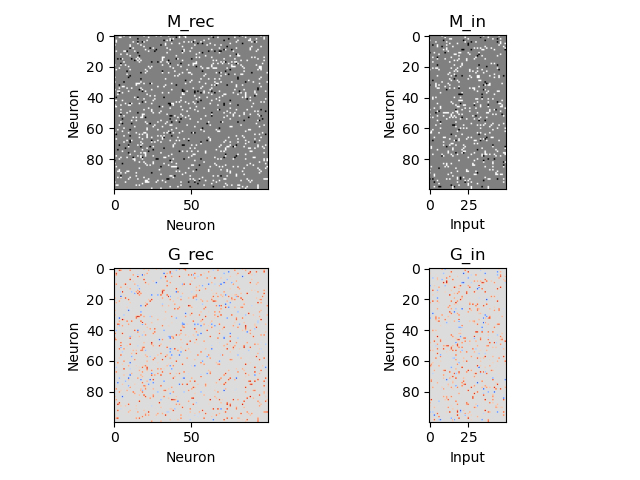
\includegraphics[scale=0.75]{Matrices}
%\end{center}


We initialize $\mathbf{A}_{0}$ from  $\mathbf{B}_{0}$ by drawing connection weights from a uniform distribution $\mathbf{A}_{0}\sim U^{n\times n}[0,g_{max}]$. 


\subsection{A general model}

Let $\mathbf{V}[I]$ be a vector recording the voltage per neuron for the duration of the simulation. We adopt the following model for the time evolution of $\mathbf{V}[I]$:

\begin{align*}
\tau_{m}\frac{d\mathbf{V}[i]}{dt} &= \sum_{n} \mathbf{I}_{n}[i]\\
&=  \sum_{n} g_{n}(\mathbf{V}[i] - E_{n})
\end{align*}

where $\mathbf{I}_{n}[J]$ is a vector of currents of class $n$ e.g., excitatory current and $E_{n}$ is the reversal potential. Using our definition of the conductance matrices in the preceding section, we have

\begin{equation}
\tau_{m}\frac{d\mathbf{V}[I]}{dt} = (\mathbf{V}[I]-E)\cdot \sum_{j} \mathbf{A}[I,j] + (\mathbf{V}[I] - E_{in})\sum_{k}\mathbf{B}[I,k])
\end{equation}

However, since $\mathbf{A}$ and $\mathbf{B}$ are not static matrices, we would need more information to write down a solution to (1). It turns out that we cannot write down a general solution since the evolution $\mathbf{A}$ and $\mathbf{B}$ is non-deterministic. To even write the update equations we need to constrain their evolution

We additionally define the \emph{observable state} matrix $\mathbf{Z}$ which is drawn at each time step from a distribution $p$ 

\begin{equation*}
p(\mathbf{Z}[i,t] = 1 | \mathbf{V}[I]) = \sigma(\mathbf{V}[I])
\end{equation*}

where $\sigma$ is a sigmoidal activation function. 

\subsubsection{Synaptic dynamics}

We begin with a naive version of synaptic plasticity, reserving the more sophisticated discussion until we have define the relevant model components. In the naive model, we consider two mechanisms by which synaptic conductances can change (i) release of neurotransmitter into the synaptic cleft and (ii) long-term potentiation and depression via spike timing. The former is a rather simple update to $\mathbf{A}$ and $\mathbf{B}$ computed from $\mathbf{Z}$

\begin{align*}
\tau_{A}\frac{d\mathbf{A}}{dt} &= -\mathbf{Z}\mathbf{A}\\
\tau_{B}\frac{d\mathbf{B}}{dt} &= -\mathbf{Z}\mathbf{B}
\end{align*}

where the initial conditions will, in general, depend on the baselines set by synaptic plasticity. For the latter criterion, we look for a Hebbian update to the conductance matrices $\mathbf{A}$ and $\mathbf{B}$ which are also derived from $\mathbf{Z}$, ignoring sub-threshold activity.

For potentiation, consider the block $\mathbf{Z}[i,t-\tau]$ where $\tau > 0$ and the vector describing recurrent inputs to neuron $i$: $\tilde{\mathbf{A}}[i,J]$. We use this vector to zero out spikes irrelevant to neuron $i$ by taking an element-wise product for each $t'\in [t-\tau, t]$

\begin{equation*}
\mathbf{U}[i,J,t] = \sum_{t-\tau}^{t} F\left( \mathbf{Z}[i,t-\tau]*\tilde{\mathbf{A}}[i,J]\right)
\end{equation*}

Similarly, for depression we use the vector describing recurrent outputs of neuron $i$

\begin{equation*}
\mathbf{U}[i,J,t] = \sum_{t-\tau}^{t} G\left( \mathbf{Z}[i,t-\tau]*\tilde{\mathbf{A}}[I,j]\right)
\end{equation*}

Computing this for all $i$ and suppressing indices allows us to write the abstract update

\begin{equation*}
\Delta \mathbf{A} = \lambda\mathbf{U} + \eta(t)
\end{equation*}

where $\eta(t) \sim P^{n\times n}$ and $P = \mathcal{N}(\mu, \sigma^{2})$ is white-noise.

\subsubsection{Information maximization}

The above equations in their general form are unlikely to be able to permit any meaningful form of learning. To rectify this, we can make use of recent postulates on efficient coding, where synaptic plasticity is the learning rule by which a network finds a solution to a rate-distortion problem [x]. Simply put, we would like to know how a network can estimate information gradients and how gradient ascent can be achieved via synaptic plasticity. In other words how does a network estimate the gradient of the following Lagrangian

\begin{equation*}
\mathbf{\mathcal{L}} = I(\tilde{R}; S) - \gamma(\tilde{R}; R)
\end{equation*}

where $R$, $\tilde{R}$ and $S$ satisy the Markov chain $S \rightarrow R \rightarrow \tilde{R}$. Maximization of the above Lagrangian provides an estimate of distribution $P(\tilde{R}|R)$. In the past decade, Williams et al. developed a method that exhaustively decomposes the Shannon information in a multivariate system in terms of the redundancy between synergies of subsets of the sources [8].
 

\subsubsection{Update equations}

\begin{equation*}
\mathbf{1}: \mathbf{V} \rightarrow \mathbb{F}_{2}^{n\times t}
\end{equation*}

Now we can write a stochastic update for the entire system

\begin{equation*}
\mathbf{V}[I,t] = \frac{\Delta t}{\tau_{m}}\left((\mathbf{V}[I,t-1]-E)\cdot \sum_{j} \mathbf{A}[I,j,t-1] + (\mathbf{V}[I,t-1] - E_{in})\cdot \sum_{k}\mathbf{B}[I,k,t-1]\right)
\end{equation*}



\section{The stimulus}

We would expect that that statistical structure of the stimulus would be causally related to the time evolution of the weight matrix $\mathbf{A}(t)$. Let the stimulus be white-noise $s \sim Q^{t}$ where $Q =  \mathcal{N}(\mu,\sigma^{2})$. We will parameterize a Poisson spike generator with an estimate of the spike rate $r(t)$ for this stimulus. To do that, we can use to generate an estimate of the spike rate using the Volterra expansion

\begin{equation*}
r(t) = r_{0} + \int_{0}^{\infty} D(\tau)s(t-\tau)d\tau
\end{equation*}

where we estimate $D(\tau)$ according to Adelson and Bergen (1985)

\begin{equation*}
D(\tau) = \alpha\exp(-\alpha\tau)\left(\frac{(\alpha\tau)^{5}}{5!}-\frac{(\alpha\tau)^{7}}{7!}\right)
\end{equation*}

and we take $\alpha=1/15$


\section*{References}

[1] Buesing et al. A spiking neuron as information bottleneck

[2] J.J. Hopfield. Neural networks and physical systems with emergent collective computational abilities

[3] Maass et al. Edge of chaos and predicting computational performance for neural circuit models

[4] Cramer et al. Control of criticality and computation in spiking neuromorphic networks with plasticity

[5] Zierenberg et al. Homeostatic plasticity and external input shape neural network dynamics

[6] Beggs et al. Universal critical dynamics in high-resolution neuronal avalanche data

[7] Chalk et al. (2019) Toward a unified theory of efficient, predictive, and sparse coding {\it PNAS}

[8] Williams et al. (2010) Nonnegative decomposition of multivariate information {\it arXiv}

[9] Bellec et al. (2020) A solution to the learning dilemma for recurrent networks for spiking neurons {\it arXiv}



\end{document}
